\documentclass[a4paper,UTF8]{article}
\usepackage{ctex}
\usepackage[margin=1.25in]{geometry}
\usepackage{color}
\usepackage{graphicx}
\usepackage{amssymb}
\usepackage{amsmath}
\usepackage{amsthm}
\usepackage{booktabs}
\usepackage{caption}
\usepackage{fancyhdr}
\usepackage{extramarks}
\usepackage{amsfonts}
\usepackage{tikz}
\usetikzlibrary{arrows}
\usepackage{algorithm}
\usepackage{algorithmicx}
\usepackage{algpseudocode}
\usepackage{listings}

%\usepackage[thmmarks, amsmath, thref]{ntheorem}
\theoremstyle{definition}
\newtheorem*{solution}{Solution}
\newtheorem*{prove}{Proof}
\usepackage{multirow}

%
% Basic Document Settings
%

\topmargin=-0.45in
\evensidemargin=0in
\oddsidemargin=0in
\textwidth=6.5in
\textheight=9.0in
\headsep=0.25in

\linespread{1.1}

\pagestyle{fancy}
\lhead{\hmwkTitle}
\chead{\hmwkClass\ (\hmwkClassInstructor\ \hmwkClassTime)}
\rhead{\hmwkAuthorName}
\lfoot{\lastxmark}
\cfoot{\thepage}

\renewcommand\headrulewidth{0.4pt}
\renewcommand\footrulewidth{0.4pt}

%
% Homework Details
%   - Title
%   - Due date
%   - Class
%   - Section/Time
%   - Instructor
%   - Author
%

\newcommand{\hmwkTitle}{Assignment \ \#3}
\newcommand{\hmwkDueDate}{September 18, 2017}
\newcommand{\hmwkClass}{Problem Solving}
\newcommand{\hmwkClassTime}{}
\newcommand{\hmwkClassInstructor}{Professor Chen}
\newcommand{\hmwkAuthorName}{李志琦 161220074}

%--

%--
\begin{document}


\subsection*{5.1-3}
\subsubsection*{a}
wrong! vertex v is on a circle, but v is a cut-vertex. Because each path from u to k will pass v



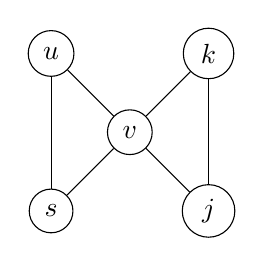
\begin{tikzpicture}
\tikzset{vertex/.style = {shape=circle,draw,minimum size=0.5em}}
\tikzset{edge/.style = {-,> = latex'}}
% vertices
\node[vertex] (s) at  (0,0) {$s$};
\node[vertex] (u) at  (0,2) {$u$};
\node[vertex] (v) at  (1,1) {$v$};
\node[vertex] (j) at  (2,0) {$j$};
\node[vertex] (k) at  (2,2) {$k$};
%edges
\draw[edge] (s) to   (u);
\draw[edge] (s) to   (v);
\draw[edge] (u) to   (v);
\draw[edge] (j) to   (v);
\draw[edge] (k) to   (v);
\draw[edge] (j) to   (k);
\end{tikzpicture}
\subsubsection*{b}
wrong! vertex u is not on any circle, but u is not a vertex obviously

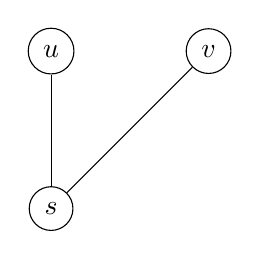
\begin{tikzpicture}
\tikzset{vertex/.style = {shape=circle,draw,minimum size=0.5em}}
\tikzset{edge/.style = {-,> = latex'}}
% vertices
\node[vertex] (s) at  (0,0) {$s$};
\node[vertex] (u) at  (0,2) {$u$};
\node[vertex] (v) at  (2,2) {$v$};
%edges
\draw[edge] (s) to   (u);
\draw[edge] (s) to   (v);
\end{tikzpicture}
\subsubsection*{c}
wrong!\\
As the graph in section b, vertex $u,v,s$ construct a tree of order 3\\
but the number of cut-vertex is 1,only s. and the number of end-vertex is 2.

\subsubsection*{d}
wrong\\
As the graph in section b, there are two edges $u-s,s-v$,but there is noly one cut-vertex.
\subsection*{5.1-4}
if v is  a cut-vertex of the complement $\bar{G}$ of $G$
then there are two vertexs $u,s$,each path bewteen them will pass $v$,\\
case 1:\\
 if $u,s$ are in different components in G, then there will be a edge between $u,s$,
so this case vill not be true.\\
case 2:\\
if $u,s$ are in same component in G,then there we can use a vertex $m$ in another componnet,
so we can  find   edges between  $u,m$, $s,m$, so there is a path between $u,s$ not pass $v$
so this case do not occur.\\
because there are only these two cases, so we know v is not a $cut\-vertex$ in graph $\bar{G}$ \\
As the graph in section b, there are two edges $u-s,s-v$,but there is noly one cut-vertex.
\subsection*{5.1-6}
1.\\
if G is 3-regular graph with a cut-vertex, so it dose'nt matter if we assume there are two components
in G-v, so we know there are two edges between vertex v and Component $G_1$, there is a edge between vertex and component
$G_2$, so this edge lies on no circle. so this edge is a bridge
2.\\
if G is 3-regular graph with a bride, from therem 5.1, since $deg v=3$, so v is a cut-vertex
\subsection*{5.2-10}
if graph G of size at least 2 is nonseparable, so let edge(u,v),and edge(v,s) be two adjacent edges ,if they are not on a common edge,
so if we remove vertex v, there will be no path between u,s. so this conflict with the graph is not noseparable graph, so any adjacent edges will lie
on common circle\\
if  any two adjacent edges of G lie on a common cycle of G. so we guess if exists two vertex u,v, each path betweent them will pass s, so we let the path be
$u\to s_1 \to s \to s_2 \v$,so we know edge($s_1$,s),edge($s_2$,s) are on a circle,
so there is a path between (u,v), not pass s ,but go through the circle exclude s, so the graph is noseparable.

\subsection*{5.2-11}
we assume the graph is not noseparable, so there is a cut-vertex v, so we may assume there are two components in graph G-v,they are $G_1,G_2$, so the maximum of the smaller order of two components is floor((n-1)/2)
the max degre of the vertex in this component is   floor((n-1)/2)(it has edge betweent each vertex in its component and vertex v),but we kow deg vertex>=n/2, so it conflicts.and assumption is wrong.
(if there are morn than two components, it is still wrong in this way)

\subsection*{5.2-14}
\subsubsection{a}
because $G_1$ is a component, so we only  nedd to show that vertex v is connected with some vertex in $V(G_1)$, because v is cut-vertex, there must be some vertex in $V(G_1)$ are adjacent to $v$
so $G(V(G_1)+v)$ is a connected graph
\subsubsection*{b}
as the graph show, if the $V(G_1)$ is w,k,j, and the cut-vertex is v, so the graph that v,w,k,j construct is not noseparable graph
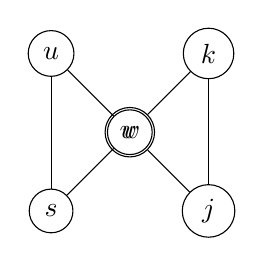
\begin{tikzpicture}
\tikzset{vertex/.style = {shape=circle,draw,minimum size=0.5em}}
\tikzset{edge/.style = {-,> = latex'}}
% vertices
\node[vertex] (s) at  (0,0) {$s$};
\node[vertex] (u) at  (0,2) {$u$};
\node[vertex] (v) at  (1,1) {$v$};
\node[vertex] (w) at  (1,1) {$w$};
\node[vertex] (j) at  (2,0) {$j$};
\node[vertex] (k) at  (2,2) {$k$};
%edges
\draw[edge] (s) to   (u);
\draw[edge] (s) to   (v);
\draw[edge] (u) to   (v);
\draw[edge] (v) to   (w);
\draw[edge] (j) to   (w);
\draw[edge] (k) to   (w);
\draw[edge] (j) to   (k);
\end{tikzpicture}
\subsection*{5.2-15}
we choose a  edge from G, so we can proof that the block found by (1) is same as the block found by (2) which they all contain edge(u,v)\\
if $block_2$ contain a edge(s,w)  called , so s,w,u,v is on common circly,so because each two vertex in (s,w,v,u) are on a common circle
so s,w,u,v  also construct a noseparable graph, this said each vertex in $block_2$ , it will lie on $block_1$\\
then as we know, each two vertexs in $block_1$ are lie on the same circle, each edge(k,m) in $block_1$ is on a circle,
,then we want to show, that this edge is on the same circle with $edge(u,v)$, so we assume, edge(k,m) and edge(u,v) is not on the same circle, then there are at least two circle in the graph and they are connected only by
a vertex, so if we remove this vertex ,this graph is disconnected, so it conflicts, and the any edge in $bolok_1$ is on the same circle as edge(u,v)
so each vertex in $bolck_1$ is in the $block_2$\\
so $block_1$ and $block_2$ are same

\subsection*{5.3-20}
\subsubsection*{a}
k=2\\
if the graph is not 2-connected, so it is 1-connected ,so vertec-cut's size is 1\\
\subsubsection*{b}

if the graph is not 2-edge-connected,since it is connected, so it is 1-edge-connected ,so vertec-cut's size is 1\\
\subsection*{5.3-22}
\subsubsection*{a}
if G -e is (k-2)-connected, so let the vertex-cut be V;
if e is incident to V,so G-V and (G-e)-V is same,so G is (k-1)-connected, contradiction.
if e is not incident to V ,so science G-V is connected (G-e)-v is disconnected,  so we can remove a vertex incident to e, so G is not connected
so G is (k-1)-connected, contradiction.
\subsubsection*{b}
if G − e is (k − 2)-edge-connected, then G is (k-1)-edge-connected, abvious wrong




\subsection*{5.3-30}
\subsection*{6.1-4}
\subsubsection*{a}
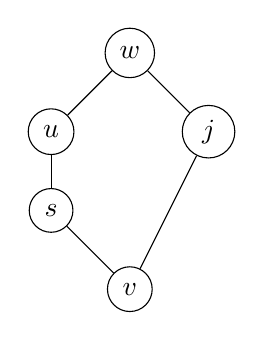
\begin{tikzpicture}
\tikzset{vertex/.style = {shape=circle,draw,minimum size=0.5em}}
\tikzset{edge/.style = {-,> = latex'}}
% vertices
\node[vertex] (s) at  (0,1) {$s$};
\node[vertex] (u) at  (0,2) {$u$};
\node[vertex] (v) at  (1,0) {$v$};
\node[vertex] (w) at  (1,3) {$w$};
\node[vertex] (j) at  (2,2) {$j$};
%edges
\draw[edge] (s) to   (u);
\draw[edge] (u) to   (w);
\draw[edge] (w) to   (j);
\draw[edge] (j) to   (v);
\draw[edge] (v) to   (s);
\end{tikzpicture}
\subsubsection*{b}
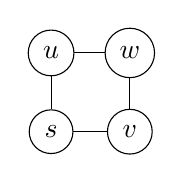
\begin{tikzpicture}
\tikzset{vertex/.style = {shape=circle,draw,minimum size=0.5em}}
\tikzset{edge/.style = {-,> = latex'}}
\node[vertex] (s) at  (0,0) {$s$};
\node[vertex] (u) at  (0,1) {$u$};
\node[vertex] (v) at  (1,0) {$v$};
\node[vertex] (w) at  (1,1) {$w$};

%edges
\draw[edge] (s) to   (u);
\draw[edge] (u) to   (w);
\draw[edge] (w) to   (v);
\draw[edge] (v) to   (s);
\end{tikzpicture}
\subsubsection*{c}
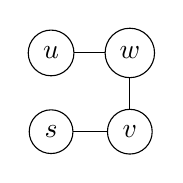
\begin{tikzpicture}
\tikzset{vertex/.style = {shape=circle,draw,minimum size=0.5em}}
\tikzset{edge/.style = {-,> = latex'}}
\node[vertex] (s) at  (0,0) {$s$};
\node[vertex] (u) at  (0,1) {$u$};
\node[vertex] (v) at  (1,0) {$v$};
\node[vertex] (w) at  (1,1) {$w$};


\draw[edge] (u) to   (w);
\draw[edge] (w) to   (v);
\draw[edge] (v) to   (s);
\end{tikzpicture}
\subsubsection*{d}

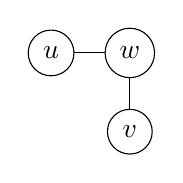
\begin{tikzpicture}
\tikzset{vertex/.style = {shape=circle,draw,minimum size=0.5em}}
\tikzset{edge/.style = {-,> = latex'}}

\node[vertex] (u) at  (0,1) {$u$};
\node[vertex] (v) at  (1,0) {$v$};
\node[vertex] (w) at  (1,1) {$w$};


\draw[edge] (u) to   (w);
\draw[edge] (w) to   (v);

\end{tikzpicture}
\subsubsection*{d}
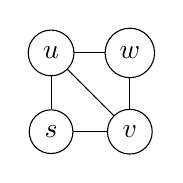
\begin{tikzpicture}
\tikzset{vertex/.style = {shape=circle,draw,minimum size=0.5em}}
\tikzset{edge/.style = {-,> = latex'}}
\node[vertex] (s) at  (0,0) {$s$};
\node[vertex] (u) at  (0,1) {$u$};
\node[vertex] (v) at  (1,0) {$v$};
\node[vertex] (w) at  (1,1) {$w$};
\draw[edge] (u) to   (s);
\draw[edge] (u) to   (v);
\draw[edge] (u) to   (w);
\draw[edge] (w) to   (v);
\draw[edge] (v) to   (s);
\end{tikzpicture}
\subsection*{6.1-5}
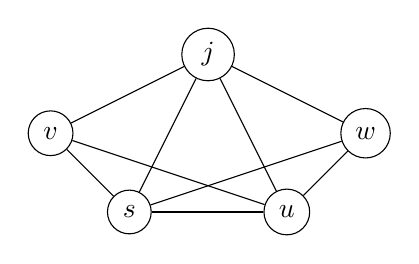
\begin{tikzpicture}
\tikzset{vertex/.style = {shape=circle,draw,minimum size=0.5em}}
\tikzset{edge/.style = {-,> = latex'}}
% vertices
\node[vertex] (s) at  (2,1) {$s$};
\node[vertex] (u) at  (4,1) {$u$};
\node[vertex] (v) at  (1,2) {$v$};
\node[vertex] (w) at  (5,2) {$w$};
\node[vertex] (j) at  (3,3) {$j$};
%edges
\draw[edge] (s) to   (w);
\draw[edge] (s) to   (j);
\draw[edge] (s) to   (u);
\draw[edge] (u) to   (w);
\draw[edge] (u) to   (v);
\draw[edge] (u) to   (j);
\draw[edge] (w) to   (j);
\draw[edge] (j) to   (v);
\draw[edge] (v) to   (s);
\end{tikzpicture}
\subsection*{6.1.6}
the graph is (2n+1) regular graph and\\
if graph is 2m-order, and $\bar{G}$ is connected, bar is even-regular graph
if graph is (2m+1)-order, it can not be a even-regulr  graph ,so it must be a Eulerian
\subsection*{6.2.13}
\subsubsection*{a}

as the graph shows, if we remove vertex s2 and s7 thne left 4 componets and 4>2,so from theorem 6.5,
this graph is not  Hamiltonian
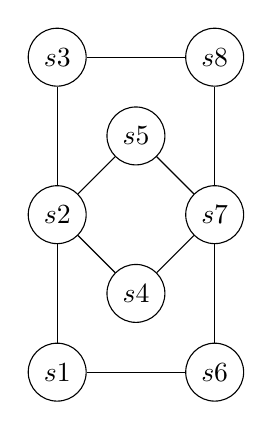
\begin{tikzpicture}
\tikzset{vertex/.style = {shape=circle,draw,minimum size=0.5em}}
\tikzset{edge/.style = {-,> = latex'}}
% vertices
\node[vertex] (s1) at  (1,1) {$s1$};
\node[vertex] (s2) at  (1,3) {$s2$};
\node[vertex] (s3) at  (1,5) {$s3$};
\node[vertex] (s4) at  (2,2) {$s4$};
\node[vertex] (s5) at  (2,4) {$s5$};
\node[vertex] (s6) at  (3,1) {$s6$};
\node[vertex] (s7) at  (3,3) {$s7$};
\node[vertex] (s8) at  (3,5) {$s8$};
%edges
\draw[edge] (s1) to   (s2);
\draw[edge] (s2) to   (s3);
\draw[edge] (s3) to   (s8);
\draw[edge] (s2) to   (s4);
\draw[edge] (s2) to   (s5);
\draw[edge] (s1) to   (s6);
\draw[edge] (s6) to   (s7);
\draw[edge] (s7) to   (s8);
\draw[edge] (s7) to   (s4);
\draw[edge] (s7) to   (s5);
\end{tikzpicture}
\subsubsection*{b}
each vertex's degree is 3, so it is not Eulerian.\\
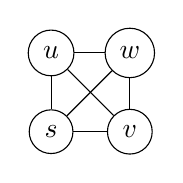
\begin{tikzpicture}
\tikzset{vertex/.style = {shape=circle,draw,minimum size=0.5em}}
\tikzset{edge/.style = {-,> = latex'}}
\node[vertex] (s) at  (0,0) {$s$};
\node[vertex] (u) at  (0,1) {$u$};
\node[vertex] (v) at  (1,0) {$v$};
\node[vertex] (w) at  (1,1) {$w$};
\draw[edge] (u) to   (s);
\draw[edge] (u) to   (v);
\draw[edge] (u) to   (w);
\draw[edge] (w) to   (v);
\draw[edge] (v) to   (s);
\draw[edge] (w) to   (s);
\end{tikzpicture}
\subsubsection*{c}
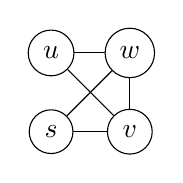
\begin{tikzpicture}
\tikzset{vertex/.style = {shape=circle,draw,minimum size=0.5em}}
\tikzset{edge/.style = {-,> = latex'}}
\node[vertex] (s) at  (0,0) {$s$};
\node[vertex] (u) at  (0,1) {$u$};
\node[vertex] (v) at  (1,0) {$v$};
\node[vertex] (w) at  (1,1) {$w$};

\draw[edge] (u) to   (v);
\draw[edge] (u) to   (w);
\draw[edge] (w) to   (v);
\draw[edge] (v) to   (s);
\draw[edge] (w) to   (s);
\end{tikzpicture}

\subsubsection*{d}

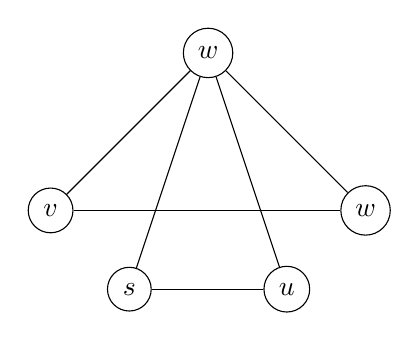
\begin{tikzpicture}
\tikzset{vertex/.style = {shape=circle,draw,minimum size=0.5em}}
\tikzset{edge/.style = {-,> = latex'}}
\node[vertex] (s) at  (2,2) {$s$};
\node[vertex] (u) at  (4,2) {$u$};
\node[vertex] (v) at  (1,3) {$v$};
\node[vertex] (w) at  (5,3) {$w$};
\node[vertex] (k) at  (3,5) {$w$};
\draw[edge] (u) to   (s);
\draw[edge] (s) to   (k);
\draw[edge] (k) to   (u);
\draw[edge] (v) to   (w);
\draw[edge] (w) to   (k);
\draw[edge] (v) to   (k);
\end{tikzpicture}
\subsection*{6.2.16}
\subsubsection*{a}

let G be r-regular, $\bar{G}$ be s-regualr,
because order of G is even, so r+s is a odd number,sience
neither r or s is 0, so there is one and only one in G and $\bar{G]}$, which is a even-regular graph,
so either G or $\bar{G}$ is Eulerian.
 \subsubsection*{b}
Corollary 6.7: Let G be a graph of order n ≥ 3. If deg v ≥ n/2 for each vertex v of G, then G is
Hamiltonian.\\
first when order is less than 3, it conficts with that both G and $\bar{G}$ is connected\\
then we let the order of G is 2n.\\
so the let G be a r-regular ,and $\bar{G}$ be a k regular.
so r+k=2n-1.\\
if neither r or k is $\gt$ n, neihter G and $\bar{G}$ will be Hamiltonian,so $r<n,k<n$,so $r+k<=2n-2$
so this is a contradiction.
so also we can proof not both r and k can not be larger  than n,so either G or is Hamiltonian.


\subsection*{6.2.21}
we can add a new vertex  s to G, and add a edge between s and each vertex in G.
so we get a new graph, G2, and eaevery two non-adjacent vertices x,y in G their degree's sum is greater than n;
so from theorem 6.6 we know G2 is Hamiltonian. so we remove the vertex s from the circle, and we get a Hamiltonian path.

\end{document}
